\documentclass[a4paper,14pt]{extreport} %размер бумаги устанавливаем А4, шрифт 14пунктов
\usepackage[T2A]{fontenc}
\usepackage{booktabs} % For prettier tables
\usepackage[utf8]{inputenc}%включаем свою кодировку: koi8-r или utf8 в UNIX, cp1251 в Windows
\usepackage[english,russian]{babel}%используем русский и английский языки с переносами
\usepackage{amssymb,amsfonts,amsmath,mathtext,cite,enumerate,float} %подключаем нужные пакеты расширений
\usepackage[dvips]{graphicx}
\usepackage{pgfplots}
%\usepackage{listings}
\usepackage[linesnumbered,boxed]{algorithm2e}
\graphicspath{{./images/}}%путь к рисункам


\makeatletter
\renewcommand{\@biblabel}[1]{#1.} % Заменяем библиографию с квадратных скобок на точку:
\makeatother

\usepackage{extsizes}

\usepackage{geometry} % Меняем поля страницы
\geometry{left=3cm}% левое поле
\geometry{right=2cm}% правое поле
\geometry{top=2cm}% верхнее поле
\geometry{bottom=2cm}% нижнее поле
\linespread{1.3}

%\renewcommand{\theenumi}{\arabic{enumi}}% Меняем везде перечисления на цифра.цифра
%\renewcommand{\labelenumi}{\arabic{enumi}}% Меняем везде перечисления на цифра.цифра
%\renewcommand{\theenumii}{.\arabic{enumii}}% Меняем везде перечисления на цифра.цифра
%\renewcommand{\labelenumii}{\arabic{enumi}.\arabic{enumii}.}% Меняем везде перечисления на цифра.цифра
%\renewcommand{\theenumiii}{.\arabic{enumiii}}% Меняем везде перечисления на цифра.цифра
%\renewcommand{\labelenumiii}{\arabic{enumi}.\arabic{enumii}.\arabic{enumiii}.}% Меняем везде перечисления на цифра.цифра


\begin{document}
\begin{titlepage}
\newpage

\begin{center}
\small МИНИСТЕРСТВО ОБРАЗОВАНИЯ И НАУКИ РОССИЙСКОЙ ФЕДЕРАЦИИ \\
\vspace{1cm}
\small ФЕДЕРАЛЬНОЕ ГОСУДАРСТВЕННОЕ АВТОНОМНОЕ ОБРАЗОВАТЕЛЬНОЕ \\*
\small УЧРЕЖДЕНИЕ ВЫСШЕГО ОБРАЗОВАНИЯ \\*
\small "МОСКОВСКИЙ ФИЗИКО-ТЕХНИЧЕСКИЙ ИНСТИТУТ \\*
\small (ГОСУДАРСТВЕННЫЙ УНИВЕРСИТЕТ)" \\*
\vspace{1cm}
\small ФАКУЛЬТЕТ ИННОВАЦИЙ И ВЫСОКИХ ТЕХНОЛОГИЙ \\*
\small КАФЕДРА ТЕОРЕТИЧЕСКИХ И ПРИКЛАДНЫХ ПРОБЛЕМ ИННОВАЦИЙ \\*
\hrulefill
\end{center}

\vspace{4em}

\begin{center}
\textbf{ВЫПУСКНАЯ КВАЛИФИКАЦИОННАЯ РАБОТА} \\
\vspace{1em}
\small \textbf{(МАГИСТЕРСКАЯ РАБОТА)} \\
\vspace{1em}
\small \textbf{Направление подготовки: 03.04.01 "Прикладные математика и физика"} \\
\vspace{1em}
\textsc{\textbf{НА ТЕМУ:}} \\
\vspace{2em}
\large \textsc{\textbf{Единая автоматизированная информационная система поддержки и сопровождения проектов, созданных с применением стандарта BIM}}
\end{center}

\vspace{6em}

\begin{flushleft}
Студент \hrulefill Княжев В.А. \\
\vspace{1em}
Научный руководитель \hrulefill Зырин С.В.\\
\vspace{1em}
%Рецензент \\
%к.ф.-м.н., в.н.с. АБВГ \hrulefill Петров В.В.\\
%\vspace{1.5em}
%Зав. кафедрой  ХХХ \\
%д.ф-м.н, профессор \hrulefill Сидоров Г.Г.
\end{flushleft}

\vspace{\fill}

\begin{center}
г. Москва, 2019
\end{center}

\end{titlepage}% это титульный лист
\tableofcontents % это оглавление, которое генерируется автоматически

\newpage
\chapter{Введение}
\section{Актуальность проблемы}

Темпы строительства зданий и промышленных объектов в мире и сложность конструкций увеличивается с каждым годом \cite{BUILDING_GROWTH_RATE}. Ранее использовавшиеся методы проектирования чертежей на бумаге отходят на второй план, и все более активно используются компьютерные технологии \cite{BUILDING_SOFTWARE}, а также становится очевидной необходимость повсеместного введения стандартов проектирования зданий. \\
Одним из наиболее современных стандартов проектирования является стандарт BIM (Building Information Modeling)\cite{BIM_FUTURE}. Его концепция позволяет не только проектировать здания, но также охватить весь их жизненный цикл: от управления затратами и строительством здания до его эксплуатации. \\
Подобная всеобъемлемость хороша тем, что вся информация о конструкции содержится в одном проекте. Это помогает сохранять целостность данных, позволяет быстрее выявлять ошибки и уменьшать стоимость ремонта. Но также из этого вытекает необходимость координации одновременной работы большого количества людей над одним проектом: крупных команд архитекторов, иногда распределенных по всему миру, эксплуатирующих организаций и всех других людей, участвующих в обслуживании здания. \\
Поэтому очень важно иметь возможность одновременного изменения BIM представления объекта разными людьми без потери каких-либо данных. Но малейшая ошибка в одном из элементов конструкции, не обнаруженная вовремя, может привести к серьезным последствиям, например к дополнительным затратам на проект. Поэтому важно в любой момент времени иметь доступ к электронному журналу аудита всех изменений проекта. \\
В настоящий момент программ, специализирующихся на архитектурных проектах стандарта BIM, и  которые бы в полной мере решали задачу по координации работы большого количества людей и отслеживания изменений, не существует. 

\newpage 
\section{Постановка задачи}

Требуется разработать веб-систему, которая бы могла предоставить пользователям следующие возможности:
\begin{enumerate}
\item Управление жизненным циклом проектов. \\
Создание проекта, добавление, редактирование  и удаление файлов, управление правами доступа к проекту.
\item Отслеживание изменений проекта во времени. \\
Отображение списка всех изменений проекта, а также возможность просмотра версии данных или внесенных в проект изменений в конкретный момент времени.
\item Одновременное внесение изменений в проекты несколькими пользователями. \\
Пользователи могут работать над разными частями проекта в одно и то же время. При наличии конфликтующих изменений предоставляется возможность сохранения изменений, внесенных как другими пользователями, так и текущим.
\item Подготовка окружения, запуск системы и ее масштабируемость. \\
Возможность быстрой подготовки окружения и запуска сервиса для мговенного развертывания веб-платформы. В моменты пиковой нагрузки пользователей, веб-платформа не должна терять производительность.
\end{enumerate}

\newpage

\chapter{Основная часть}
\section{Стандарт BIM}


\newpage
\section{Формат данных}


\newpage
\section{Пользовательские истории}

Пользовательские истории (user story) -- способ описания требований к разрабатываемому продукту, которые сформулированы на понятном пользователю языке. Каждая пользовательская история должна быть ограничена в размере и сложности ее реализации. \\
Пользовательские истории -- быстрый способ документирования основных требований клиента, их целью является оперативное регирование на изменения требований реального мира. \\
Текст каждой пользовательской истории должен пояснять роль пользователя и его действия в системе. Для начала требуется определить список основных пользователей нашей системы.

\subsection{Набор персонажей}

Для получения конечного списка персонажей воспользуемся иерархическо кластеризацией. Требуется составить список протоперсонажей (персонажей-гипотез), создать список шкал умений, поведенческих и мотивационных переменных. Далее, с помощью кластеризации персонажей по ранее составленным критериям (в данной работе проводится кластеризация с помощью дендограмм), проанализировать первоначальный список персонажей и сократить его до самых значимых.

\subsubsection{Персонажи-гипотезы}
\begin{enumerate}
\item Архитектор
\item Главный архитектор
\item Дизайнер
\item Студент технического направления
\item Инвестор
\item Строитель
\end {enumerate}

\subsubsection{Умения, поведенческие и мотивационные переменные}

Выделены следующие характеристики, в той или иной мере описывающие наших персонажей-прототипов.
\begin{enumerate}
\item Уровень технического образования \\
1 - законченная средняя школа, 5 - PhD
\item Знание иностранных языков \\
1 - beginner, 5 - proficiency
\item Опыт работы с персональными компьютерами \\
1 - обычный пользователь, 5 - администратор ПК
\item Цели использования нашей системы \\
1 - протестировать систему, 5 - коммерческое использование
\item Частота использования нашей системы \\
1 - единичное использование, 5 - постоянное взаимодействие с системой
\item Масштабы создаваемых проектов \\
1 - домашние маленькие проекты, 5 - проекты крупных зданий
\item Умение проектировать архитектурные модели \\
1 - нет опыта, 5 - опыт более 5 лет и профессиональное образование
\item Платежеспособность \\
1 - отсутствие постоянного дохода, 5 - наличие крупных бизнесов
\end{enumerate}

\newpage
\subsubsection{Матрица сходства персонажей}

В данной матрице в первом столбце перечислены все персонажи-прототипы, в первой строке перечислены номера  указанных выше описательных характеристик.

\begin{table}[H]
\caption {Матрица  сочетаний персонажей и характеристик} \label{tab:title}
\begin{center}
\begin{tabular}{| p{4cm}  | p{1cm} | p{1cm} | p{1cm} | p{1cm} | p{1cm} | p{1cm} | p{1cm} | p{1cm} |}
\hline
\textbf{Персонаж} & \textbf{1} & \textbf{2} & \textbf{3} & \textbf{4} & \textbf{5} & \textbf{6} & \textbf{7} & \textbf{8} \\
\hline
Архитектор 		& 4 & 2 & 3 & 4 & 4 & 4 & 4 & 3 \\
\hline
Гл. архитектор	& 5 & 5 & 4 & 5 & 5 & 5 & 5 & 4 \\
\hline
Дизайнер			& 3 & 2 & 3 & 3 & 3 & 2 & 3 & 3 \\
\hline
Студент			& 3 & 2 & 3 & 2 & 2 & 2 & 3 & 1 \\
\hline
Инвестор			& 4 & 5 & 4 & 5 & 2 & 5 & 1 & 5 \\
\hline
Строитель		& 2 & 1 & 2 & 3 & 3 & 4 & 2 & 2 \\
\hline
\end{tabular}
\end{center}
\end{table}

\subsubsection{Построение дендограммы}

Под дендрограммой понимается дерево, которое построено на основе матрицы мер близости. Она позволяет отобразить взаимные связи между объектами из первоначально заданного множества объектов. Для построения дендрограммы требуется составить матрицу сходства, которая определяет уровень сходства между парами кластеров. \\
При построении дендограмм могут использоваться следующие способы кластеризации данных:
\begin{itemize}
\item {\it Агломеративные методы} \\
Когда новые кластеры создаются путем объединения более мелких кластеров, дерево строится от листьев к корню.
\item {\it Дивизивные или дивизионные методы} \\
Когда более крупные кластеры делятся на более мелкие, дерево строится от корня к листьям.
\end{itemize}
В данной работе используется агломеративный метод, а именно метод одиночной связи (ближайшего соседа).
Расстояние между двумя различными кластерами берется равным минимальному расстоянию между двумя элементами из них
\textit{
\begin{equation}
\label{dendogramm_algo}
 dist(\mathcal{A},\mathcal{B}) = min \{ d(a, b) : a \in \mathcal{A}, b \in \mathcal{B} \}
\end{equation}
где $d(a, b)$ -- расстояние между элементами $a$ и $b$, принадлежащими кластерам $\mathcal{A}$ и $\mathcal{B}$ 
}

\begin{figure}[H]
\center{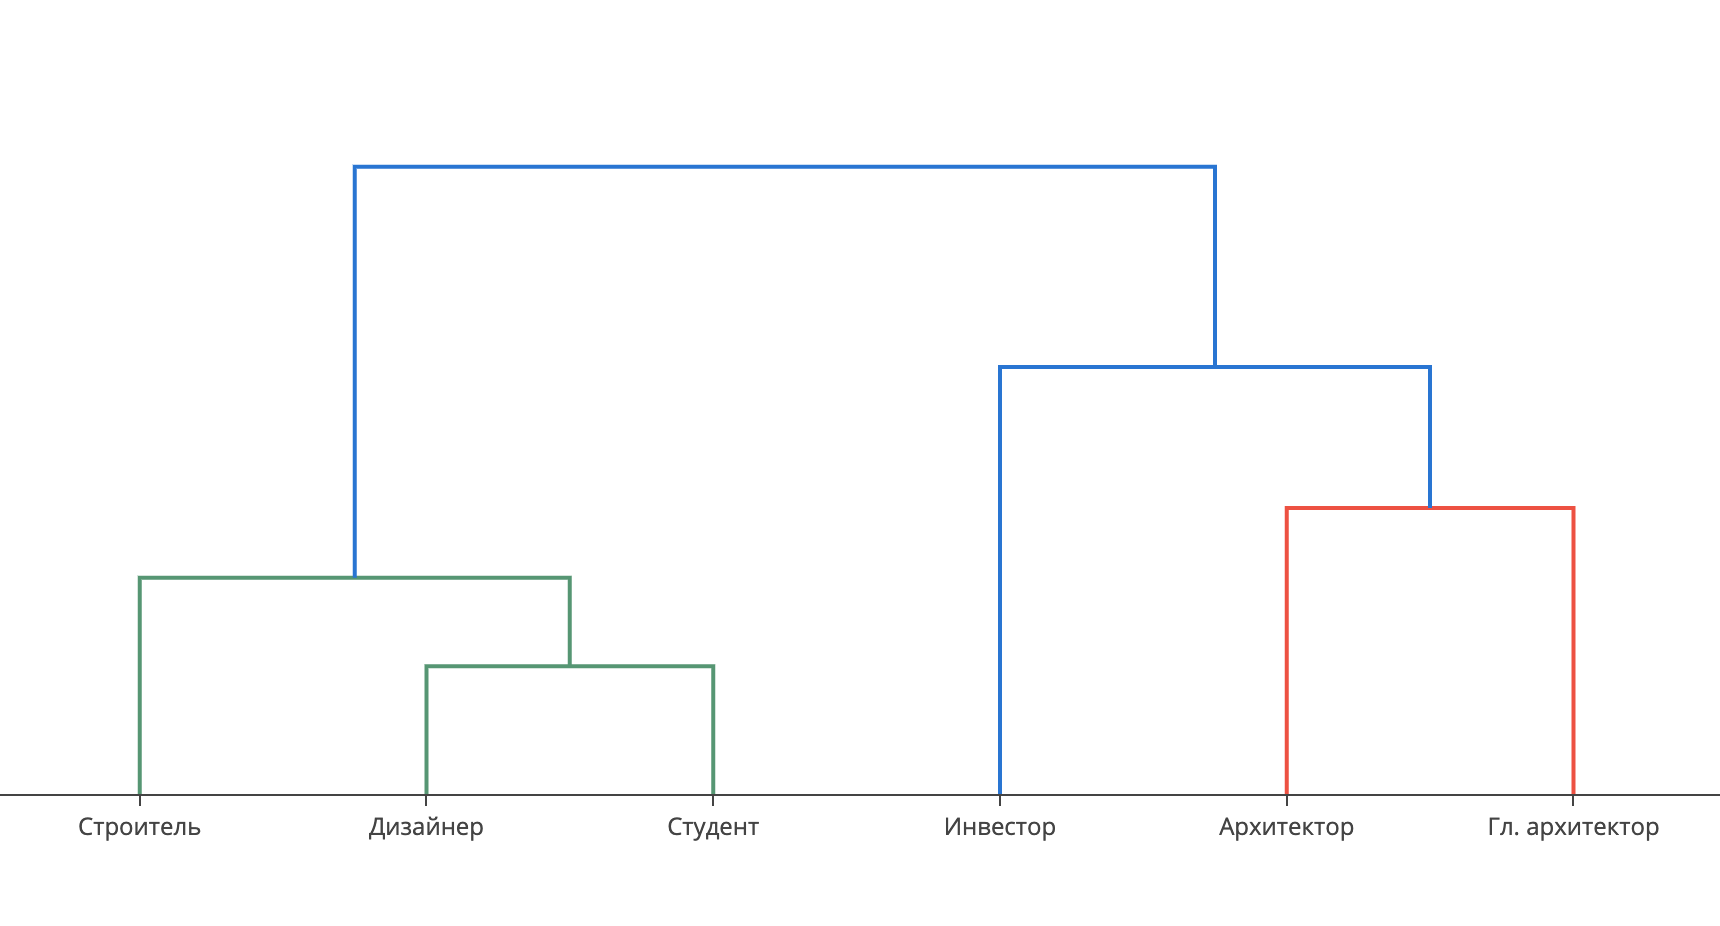
\includegraphics[width=1.0\textwidth]{dendogramm.png}}
\caption{Дендограмма.}
\label{user-stories}
\end{figure}

\subsubsection{Итоговый набор персонажей}

Конечный набор персонажей, которые будут анализироваться в данной работе, представлен ниже:
\begin{itemize}
\item Главный архитектор
\item Архитектор
\item Куратор проекта
\item Строитель
\end{itemize}

Куратором проекта в данном случае является любое лицо, которое желает следить за процессом разработки архитектурных проектов, например, инвестор.

\newpage
\subsection{Действия пользователей}

Описанные в разделе ранее пользователи имеют следующие цели при работе с нашей системой, а также планируют выполнять определенные действия с некоторыми ограничениями.

\subsubsection{Главный архитектор}

\textit{Личные цели:}
\begin{enumerate}
\item Управление жизненным циклом проекта
\item Контроль над процессом разработки проекта
\item 
\end{enumerate}

\textit{Действия}
\begin{enumerate}
\item 
\end{enumerate}

\textit{Требования}
\begin{enumerate}
\item 
\end{enumerate}

\subsubsection{Архитектор}

\textit{Личные цели:}
\begin{enumerate}
\item 
\end{enumerate}

\textit{Действия}
\begin{enumerate}
\item 
\end{enumerate}

\textit{Требования}
\begin{enumerate}
\item 
\end{enumerate}

\subsubsection{Куратор}

\textit{Личные цели:}
\begin{enumerate}
\item 
\end{enumerate}

\textit{Действия}
\begin{enumerate}
\item 
\end{enumerate}

\textit{Требования}
\begin{enumerate}
\item 
\end{enumerate}

\subsubsection{Строитель}

\textit{Личные цели:}
\begin{enumerate}
\item 
\end{enumerate}

\textit{Действия}
\begin{enumerate}
\item 
\end{enumerate}

\textit{Требования}
\begin{enumerate}
\item 
\end{enumerate}

\subsection{Карта пользовательских историй}

\begin{figure}[H]
\center{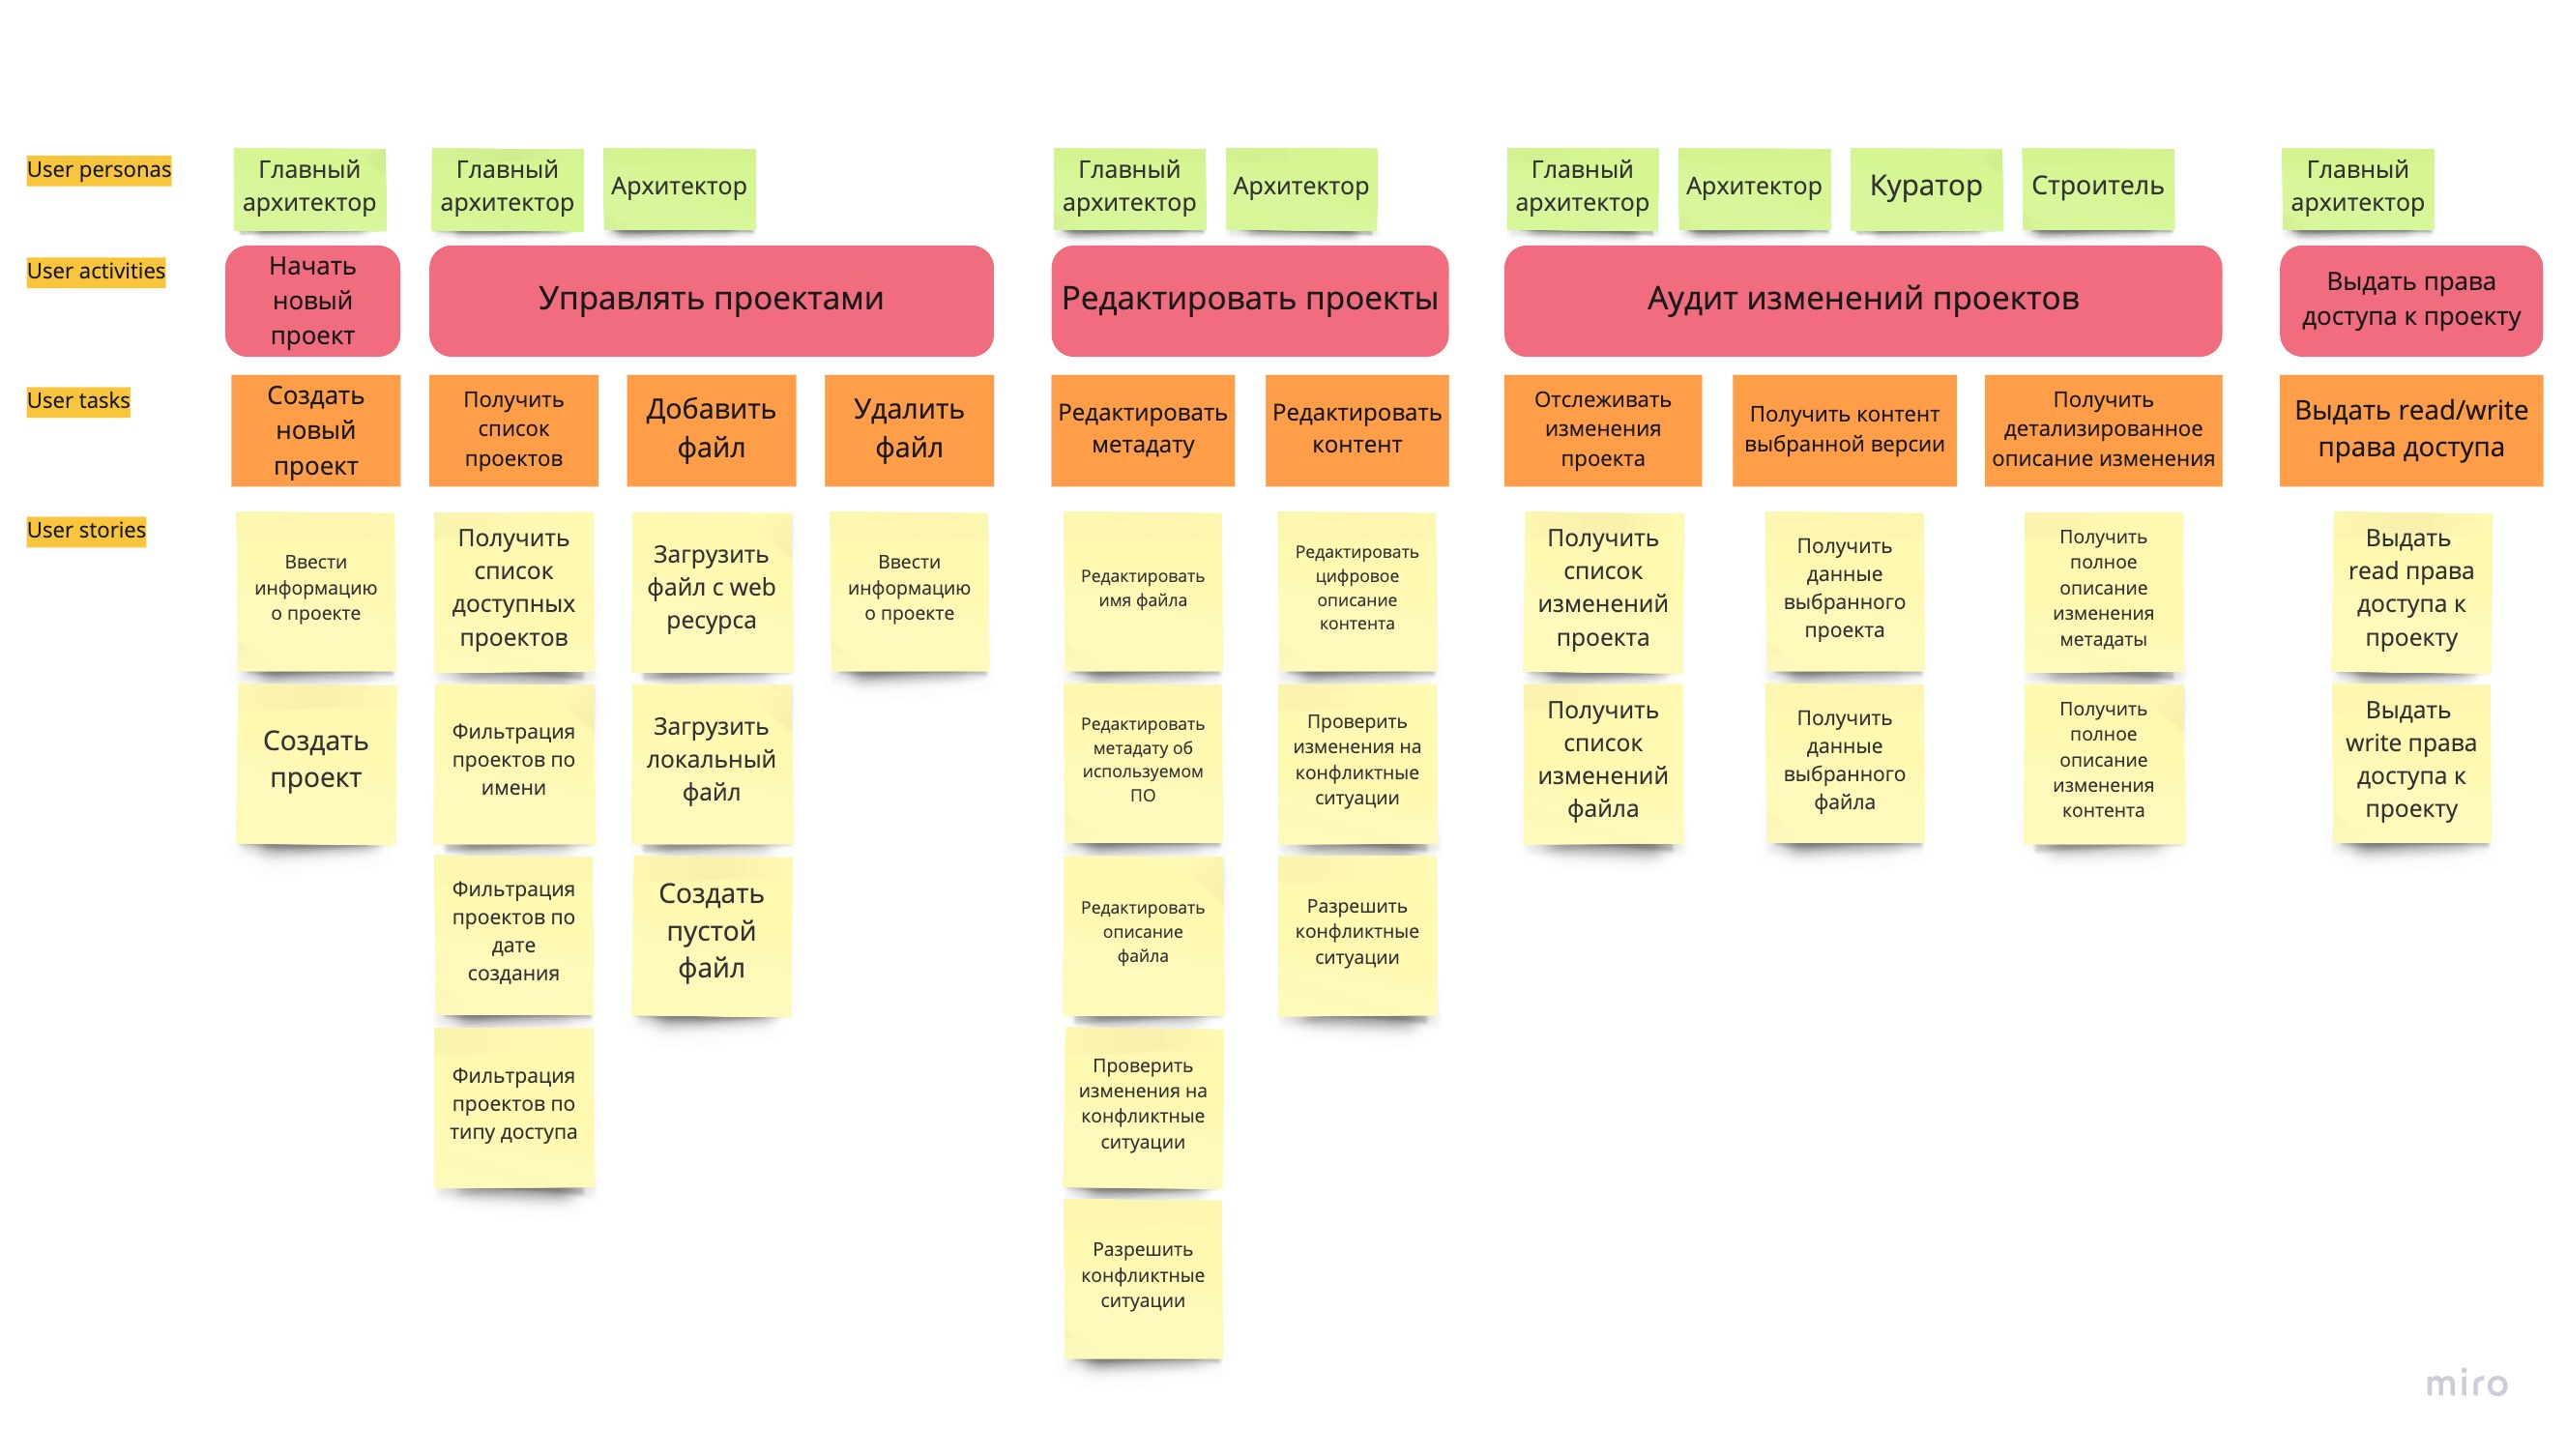
\includegraphics[width=1.0\textwidth]{user-story-mapping.jpg}}
\caption{Пользовательские истории.}
\label{user-stories}
\end{figure}

\newpage
\section{Бизнес-требования}

Бизнес-требования (business requirements) -- информация, в совокупности описывающая потребность, которая инициирует один или больше проектов с целью предоставить решение и получить требуемый конечный результат. В основу бизнес-требований ложатся бизнес-возможности, бизнес-цели, критерии успеха и положение о концепции. \\
Бизнес-требования определяют концепцию решения и границы проекта, в котором оно будет реализовываться. \\
Концепция и границы -- два базовых элемента бизнес-требований. \\ Концепция продукта (product vision) должна кратко описывать конечный продукт, который в свое время должен достигать заданных бизнес-целей. \\
Границы проекта (project scope) показывают, какая часть конечной концепции продукта будет реализована в текущей итерации. \\
В данной работе границы проекта совпадают с концепцией решения. \\
Документ о концепции и границах (vision and scope document) -- единый документ, который включает в себя все бизнес-требования. \\
Далее будут представлены основные пункты этого документа.

\subsection{Исходные данные}

На данный момент архитекторам требуется веб-платформа для одновременной работы с архитектурными проектами без потери данных, которая также предоставляла бы доступ к электронному журналу аудита всех изменений проектов.

\newpage
\subsection{Бизнес-цели}

\begin{table}[H]
\caption {Нефинансовые цели} \label{tab:title}
\begin{center}
\begin{tabular}{ | l | p{14cm} | }
\hline
№ & Цель \\
\hline
Н1 & Разработать веб-платформу для управления жизненным циклом	архитектурных проектов \\
\hline
Н2 & Реализовать возможность одновременного редактирования проектов и разрешения конфликтов в случаях их наличия \\
\hline
Н3 & Реализовать хранение журнала аудита всех изменений проектов и возможность его просмотра \\
\hline
\end{tabular}
\end{center}
\end{table}
 
\subsection{Критерии успеха}

\begin{itemize}
\item Веб-платформа позволяет управлять жизненным циклом архитектурного проекта.
\item Веб-платформе предоставляет возможность просмотра электронного журнала аудита изменений проекта.
\item Веб-платформа позволяет разрешать конфликты, возникающие при одновременном редактировании, без потери данных.
\end {itemize}
 
 \subsection{Положение о концепции проекта}
 
Для пользователей, которым требуется управлять жизненным циклом  архитектурных проектов и иметь возможность отслеживать изменения  во времени, данная работа является веб-платформой, которая будет выступать в качестве единой системы по хранению и изменению архитектурных проектов без потери данных с возможностью просмотра электронного журнала аудита изменений.

\newpage
\section{Ограничения системы}
\subsection{Основные функции}

\begin{enumerate}
\item Просмотр списка доступных пользователю проектов.
\item Создание проекта.
\item Управление правами доступа к проекту.
\item Добавление файлов в проект.
\item Изменение метадаты проекта и его файлов.
\item Удаление файла из проекта.
\item Просмотр контента файла.
\item Редактирование контента файла.
\item Просмотр журнала аудита изменений проекта.
\item Просмотр контента проекта в определенный промежуток времени.
\item Просмотр списка изменений, внесенных в проект в определенный момент времени.
\item Разрешение конфликтных ситуаций при редактировании файлов проекта.
\end {enumerate}

\subsection{Ограничения и исключения}

\begin{itemize}
\item Размер каждого файла должен не превышать 150 Мб (ограничение IFC формата).
\item В данной работе не предполагается возможность создания файлов со связанными между собой BIM представлениями объектов.
\end {itemize}

\newpage

\section{Функции системы}

\begin{enumerate}

\item Просмотр списка проектов

\begin{table}[H]
\caption {Просмотр списка проектов} \label{tab:title}
\begin{center}
\begin{tabular}{| p{2.5cm}  | p{11.5cm} |}
\hline
Описание & Пользователь может просмотреть список доступных ему преоктов. Также для поиска проектов имеется возможность фильтрации данных. \\
\hline
\multicolumn{2}{ | l | }{Функциональные требования:} \\
\hline
ПСПФ1 & Система должна предоставить список всех проектов по заданным фильтрам  \\
\hline
ПСПФ2 & Записи проектов должны содержать следующую информацию: имя, описание проекта, даты создания и последнего изменения, имя владельца, а также краткую информацию о файлах. \\
\hline
\multicolumn{2}{ | l | }{Нефункциональные требования:} \\
\hline
ПСПН1 & Пользователю отображаются только те проекты, владельцем которых он является, или к которым он имеет доступ на чтение или редактирование .\\
\hline
\end{tabular}
\end{center}
\end{table}

\newpage

\item Создание проекта \\

\begin{table}[H]
\caption {Создание проекта} \label{tab:title}
\begin{center}
\begin{tabular}{| p{2.5cm}  | p{11.5cm} |}
\hline
Описание & Создание проекта с указанием его названия и описания. \\
\hline
\multicolumn{2}{ | l | }{Функциональные требования:} \\
\hline
СПФ1 & При создании проекта система должна предоставить пользователю идентификатор, по которому он теперь сможет работать с только что созданным проектом. \\
\hline
СПФ2 & При создании проекта система предоставляет пользователю возможность ввести имя и описание нового проекта. \\
\hline
\end{tabular}
\end{center}
\end{table}

\item Управление правами доступа к проекту \\

\begin{table}[H]
\caption {Управление правами доступа} \label{tab:title}
\begin{center}
\begin{tabular}{| p{2.5cm}  | p{11.5cm} |}
\hline
Описание & Предоставление доступа к проекту другим пользователям \\
\hline
\multicolumn{2}{ | l | }{Функциональные требования:} \\
\hline
ПДФ1 & Каждому пользователю можно выдать права доступа к проекту  \\
\hline
\multicolumn{2}{ | l | }{Нефункциональные требования:} \\
\hline
ПДН1 & Права пользователей подразделяются на чтение, редактирование. Права на чтение подразумевают только просмотр всех данных проекта и его изменений. Права на редактирование включают в себя права на чтение, а также возможность управлять жизненным циклом проекта. \\
\hline
ПДН2 & Только владелец проекта имеет возможность предоставлять какие-либо права доступа к проекту. \\
\hline
ПДН3 & По умолчанию новый проект доступен только его владельцу. \\
\hline
\end{tabular}
\end{center}
\end{table}

\item Добавление файлов в проект \\

\begin{table}[H]
\caption {Добавление файлов в проект} \label{tab:title}
\begin{center}
\begin{tabular}{| p{2.5cm}  | p{11.5cm} |}
\hline
Описание & В уже созданный проект происходит добавление нового файла с контентом. Загружаться данные могут как по ссылке, так и самим файлом с данными. Также файлы можно удалять. \\
\hline
\multicolumn{2}{ | l | }{Функциональные требования:} \\
\hline
ДФФ1 & При невозможности загрузить данные система должна оповестить об этом пользователя (с указанием причины) \\
\hline
ДФФ2 & Для удаления файла из проекта система требует указание его идентификатора и повторное подтверждение запроса на удаление \\
\hline
ДФФ3 & При удалении файла из проекта система отображает этот файл только пользователям, имеющим права на редактирование \\
\hline
\multicolumn{2}{ | l | }{Требования к данным:} \\
\hline
ДФД1 & Формат загружаемых данных должен соответствовать стандарту IFC \\
\hline
ДФД2 & Максимальный размер загружаемых данных - 150 Мб \\
\hline
\end{tabular}
\end{center}
\end{table}

\item Редактирование контента файла \\

\begin{table}[H]
\caption {Редактирование контента файла} \label{tab:title}
\begin{center}
\begin{tabular}{| p{2.5cm}  | p{11.5cm} |}
\hline
Описание & Пользователь имеет возможность изменить контент неудаленных файлов в проектах. \\
\hline
\multicolumn{2}{ | l | }{Функциональные требования:} \\
\hline
ВИФ1 & После внесения изменений в контент текущей версии файла система должна проверить корректность данного изменения и оповестить пользователя либо о невозможности выполнения, либо об успешности операции \\
\hline
ВИФ2 & После внесения изменений в контент файла система должна обновить историю проекта \\
\hline
\multicolumn{2}{ | l | }{Нефункциональные требования:} \\
\hline
ВИН1 & Вносить изменения разрешается только в неудаленные файлы \\
\hline
\end{tabular}
\end{center}
\end{table}

\end {enumerate}


\newpage
\section{Описание системы}


\newpage
\section{Описание алгоритмов}


\newpage
\section{Инфраструктура веб-платформы}


\newpage
\section{Характеристики качества}


\newpage
\chapter{Заключение}

\begin{thebibliography}{1}
{\small
\bibitem{BUILDING_GROWTH_RATE} {\it GlobalData.}
\textbf{Global construction output growth to reach 3.4\% in 2019} // Публикация на www.globaldata.com. 11 April 2019.
\bibitem{BUILDING_SOFTWARE} {\it Author1, Author2.}
\textbf{The name of example} // conference of this article. 2019. pp. 45-49
\bibitem{BIM_FUTURE} {\it Karen M. Kensek, Douglas E. Noble.}
\textbf{Building Information Modeling: BIM in Current and Future Practice (1st ed.)} // 2014 Hoboken, New Jersey: John Wiley
\bibitem{BIB_EXAMPLE} {\it Author1, Author2.}
\textbf{The name of example} // conference of this article. 2019. pp. 45-49
}
\end{thebibliography}

\end{document}
